% ============================================================================
% DOCUMENTO PRINCIPAL - Informe Técnico de Proyecto Final
% Universidad Nacional del Altiplano - Puno
% Curso: Sistemas de Recomendación
% ============================================================================

% ============================================================================
% PREÁMBULO - Configuraciones y Paquetes
% ============================================================================

% Clase de documento
\documentclass[12pt,oneside]{book}

% -------------------------------------------------------------------------
% Paquetes fundamentales
% -------------------------------------------------------------------------

% Idioma español - Traducir "Cuadro" como "Tabla"
\usepackage[spanish]{babel}
\addto\captionsspanish{\def\tablename{Tabla}}

% Codificación UTF-8
\usepackage[utf8]{inputenc}

% Paquete para ecuaciones matemáticas
\usepackage{amsmath}
\usepackage{amssymb}

% Times New Roman (simula la fuente)
\usepackage{mathptmx}

% Interlineado 1.5
\usepackage{setspace}
\setstretch{1.5}

% Márgenes: Izquierdo 3.0 cm, Superior/Inferior/Derecho 2.5 cm
\usepackage{geometry}
\geometry{
    left=3.0cm,
    right=2.5cm,
    top=0.5cm,
    bottom=2.5cm
}

% -------------------------------------------------------------------------
% Paquetes adicionales
% -------------------------------------------------------------------------

% Control de líneas huérfanas/viudas
\widowpenalty=10000
\clubpenalty=10000

% Saltos de página controlados
\usepackage{emptypage}

% Formato de encabezados y pies de página
\usepackage{fancyhdr}
\fancyhf{}
\fancyhead[C]{}
\fancyfoot[C]{\thepage}
\pagestyle{fancy}

% Sangría francesa (primera línea)
\usepackage{indentfirst}

% URLs en bibliography
\usepackage{url}

% Hipervínculos en el PDF
\usepackage[colorlinks=true,linkcolor=black,anchorcolor=black,citecolor=black,filecolor=black,urlcolor=black]{hyperref}

% -------------------------------------------------------------------------
% Bibliografía - APA 7ma Edición (definida, uso manual)
% -------------------------------------------------------------------------
% Para habilitar citas automáticas: usar \cite{clave}
% \usepackage[backend=biber,style=apa,sorting=nyt]{biblatex}
% \addbibresource{referencias/bibliografia.bib}

% -------------------------------------------------------------------------
% Configuración de tablas y figuras
% -------------------------------------------------------------------------

\usepackage{graphicx}
\graphicspath{{figuras/}}

\usepackage{float}
\usepackage{array}
\usepackage{tabularx}
\usepackage{booktabs}
\usepackage[labelfont=bf]{caption}

% -------------------------------------------------------------------------
% Configuración de numeración de capítulos
% -------------------------------------------------------------------------

\usepackage{titlesec}

% Capítulo: "CAPÍTULO I"
\titleformat{\chapter}[display]
    {\bfseries\Large\centering}
    {\MakeUppercase{CAPÍTULO \Roman{chapter}}}
    {20pt}
    {\MakeUppercase}
    []

% Sección 1.1, 1.2 - justificada a la izquierda
\titleformat{\section}
    {\bfseries\large\raggedright}
    {\thesection}
    {0.5em}
    {}

% Subsección 1.1.1 - justificada a la izquierda
\titleformat{\subsection}
    {\bfseries\normalsize\raggedright}
    {\thesubsection}
    {0.5em}
    {}

% Paquete para bloques de código
\usepackage{listings}
\usepackage{xcolor}

\definecolor{codegreen}{rgb}{0,0.6,0}
\definecolor{codegray}{rgb}{0.5,0.5,0.5}
\definecolor{codepurple}{rgb}{0.58,0,0.82}
\definecolor{backcolour}{rgb}{0.96,0.96,0.98}

\lstdefinestyle{mystyle}{
    backgroundcolor=\color{backcolour},   
    commentstyle=\color{codegreen},
    keywordstyle=\color{magenta},
    numberstyle=\tiny\color{codegray},
    stringstyle=\color{codepurple},
    basicstyle=\ttfamily\footnotesize,
    breakatwhitespace=false,         
    breaklines=true,                 
    captionpos=b,                    
    keepspaces=true,                 
    numbers=left,                    
    numbersep=5pt,                  
    showspaces=false,                
    showstringspaces=false,
    showtabs=false,                  
    tabsize=2
}
\lstset{style=mystyle}

\begin{document}

% ----- PÁGINAS PRELIMINARES -----
\pagenumbering{roman}

% Portada Institucional
\thispagestyle{empty}
\begin{titlepage}

\thispagestyle{empty}

% Bloque 1: Institución
\begin{center}
    \Large\textbf{UNIVERSIDAD NACIONAL DEL ALTIPLANO - PUNO} \\[0.3cm]
    \Large\textbf{FACULTAD DE INGENIERÍA MECÁNICA ELÉCTRICA, ELECTRÓNICA Y SISTEMAS} \\[0.3cm]
    \Large\textbf{ESCUELA PROFESIONAL DE INGENIERÍA DE SISTEMAS}
\end{center}

\vspace{0.4cm}

% Bloque 2: Logo institucional
\begin{center}
    
\includegraphics[width=4.5cm]{figuras/Logo_UNAP.png}
\end{center}

\vspace{0.4cm}

% Bloque 3: Título del Proyecto
\begin{center}
    \Large\textbf{PROYECTO FINAL: DESARROLLO DE UNA APLICACIÓN DE SISTEMA DE RECOMENDACIÓN HÍBRIDO DE LAPTOPS} \\[0.3cm]
    \normalsize CURSO: SISTEMAS DE RECOMENDACIÓN
\end{center}

\vspace{0.6cm}

% Bloque 4: Autor
\begin{center}
    \normalsize PRESENTADO POR: \\[0.2cm]
    \large\textbf{CARMEN NIEVES APAZA CONDORI}
\end{center}

\vspace{0.6cm}

% Bloque 5: Nivel
\begin{center}
    \normalsize INFORME TÉCNICO DE APLICACIÓN FUNCIONAL Y EVALUACIÓN DE MODELOS
\end{center}

% Bloque 6: Lugar y Fecha
\vfill

\begin{center}
    PUNO - PERÚ \\
    2026
\end{center}

\end{titlepage}
\clearpage

% Resumen / Abstract
\thispagestyle{plain}
\chapter*{Resumen}
\addcontentsline{toc}{chapter}{Resumen}

El presente proyecto reporta el diseño, desarrollo, implementación y evaluación científica de un **Sistema de Recomendación Híbrido en Dos Niveles** para computadoras portátiles (laptops), concebido para mitigar los problemas de escasez de datos (*data sparsity*) e inicio en frío (*cold start*). La arquitectura integra un **Filtro Estricto por Reglas de Dominio en Cascada** ($M_{rules}$) en el Nivel 1, seguido de un **Ensamble Ponderado Dinámico** en el Nivel 2 que combina: (i) Teoría de Utilidad Multi-Atributo (**MAUT**) basada en modelos de conocimiento de hardware, (ii) Factorización Matricial **SVD** (*Singular Value Decomposition*) para filtrado colaborativo, y (iii) Filtrado Basado en Contenido mediante similitud de coseno vectorial (**TF-IDF**). 

La plataforma web fue desarrollada utilizando **FastAPI** como backend de alta velocidad y un frontend interactivo en **HTML5, CSS3 Vanilla, JavaScript ES6+ y Chart.js**, incorporando características de grado comercial como comparador cara a cara (1vs1), selector multimoneda (USD, PEN, EUR), insignias de relación calidad/precio (*Value Score*), filtros de estilo de vida (*lifestyle tags*) y vinculación directa con ofertas en vivo de Amazon. La evaluación experimental sobre un catálogo de 150 laptops y 1,999 calificaciones demostró un rendimiento óptimo con un **$RMSE = 1.0503$**, una robustez del **$100\%$ en $CSR@10$** ante usuarios nuevos, y una **$Precision@10 = 100\%$**, consolidando una solución integral y de alto impacto para el comercio electrónico.

\vspace{0.8cm}
\noindent \textbf{Palabras Clave:} Sistemas de Recomendación Híbridos, Factorización Matricial SVD, MAUT, Inicio en Frío, FastAPI, Chart.js.

\clearpage

\chapter*{Abstract}
\addcontentsline{toc}{chapter}{Abstract}

This project reports the design, development, implementation, and scientific evaluation of a **Two-Level Hybrid Recommender System** for laptop computers, engineered to mitigate data sparsity and cold start problems. The architecture integrates a **Cascaded Domain Rule Mask** ($M_{rules}$) at Level 1, followed by a **Dynamic Weighted Ensemble** at Level 2 combining: (i) Multi-Attribute Utility Theory (**MAUT**) based on domain knowledge models, (ii) **SVD** Matrix Factorization for collaborative filtering, and (iii) Content-Based Filtering via vector cosine similarity (**TF-IDF**).

The web platform was built using **FastAPI** as a high-speed backend and an interactive frontend with **HTML5, Vanilla CSS3, JavaScript ES6+, and Chart.js**, incorporating commercial-grade features such as a 1vs1 head-to-head comparison tool, multi-currency selector (USD, PEN, EUR), value score badges, lifestyle filters, and direct Amazon store offer integration. Experimental evaluation over a catalog of 150 laptops and 1,999 ratings demonstrated optimal performance with **$RMSE = 1.0503$**, **$100\%$ $CSR@10$** robustness under cold start scenarios, and **$100\%$ $Precision@10$**, establishing a high-impact solution for modern e-commerce environments.

\vspace{0.8cm}
\noindent \textbf{Keywords:} Hybrid Recommender Systems, SVD Matrix Factorization, MAUT, Cold Start, FastAPI, Chart.js.

\clearpage

% Índice General (Tabla de contenidos)
\thispagestyle{plain}
\tableofcontents
\addcontentsline{toc}{chapter}{Índice General}
\clearpage

% Índice de Tablas
\thispagestyle{plain}
\listoftables
\addcontentsline{toc}{chapter}{Índice de Tablas}
\clearpage

% Índice de Figuras
\thispagestyle{plain}
\listoffigures
\addcontentsline{toc}{chapter}{Índice de Figuras}
\clearpage

% ----- CONTENIDO PRINCIPAL -----
\clearpage
\pagenumbering{arabic}

% Capítulo I: Introducción
\chapter{Introducción}

\section{Contexto del Proyecto}
En la era digital actual, el comercio electrónico de bienes tecnológicos experimenta un crecimiento exponencial. Sin embargo, la compra de computadoras portátiles (laptops) representa una decisión de alta complejidad cognitiva para los usuarios debido a la abundancia de especificaciones técnicas heterogéneas (microarquitectura de CPU, núcleos, memoria RAM, aceleradores GPU, potencia de VRAM, pantallas OLED/4K y soporte CUDA). 

Los algoritmos de filtrado colaborativo tradicionales (*Collaborative Filtering*) sufren de limitaciones severas en este dominio, principalmente la escasez de datos (*data sparsity*) y el problema del inicio en frío (*cold start*), en el cual usuarios nuevos sin historial previo de calificaciones no pueden recibir sugerencias relevantes.

\section{Planteamiento del Problema}
Actualmente, los portales web de e-commerce convencionales dependen de buscadores por palabras clave o filtros manuales rígidos que no consideran la compensación multidimensional entre presupuesto, rendimiento y portabilidad. Las principales deficiencias identificadas son:
\begin{enumerate}
    \item \textbf{Recomendaciones irrelevantes para usuarios nuevos}: Los modelos puramente colaborativos fallan al no disponer de interacción previa del usuario.
    \item \textbf{Violación de restricciones de hardware incompatibles}: Recomendar una laptop sin GPU dedicada a un usuario que requiere ejecutar modelos de Deep Learning o renderizado 3D genera insatisfacción crítica.
    \item \textbf{Opacidad en la justificación}: Los usuarios no comprenden por qué un modelo específico es sugerido, careciendo de métricas de relación calidad/precio o comparativas directas.
\end{enumerate}

\section{Justificación}
El desarrollo de un **Sistema de Recomendación Híbrido** que combine modelos basados en conocimiento explícito, teoría de decisión multicriterio (MAUT), factorización matricial (SVD) y similitud de contenido vectorial permite superar de forma integral las deficiencias mencionadas. Esta arquitectura garantiza que:
\begin{itemize}
    \item El usuario reciba recomendaciones 100\% válidas mediante filtrado por reglas en cascada.
    \item El sistema responda de manera óptima tanto a usuarios con historial de calificaciones previo como a usuarios nuevos (*Cold Start*).
    \item Se disponga de una interfaz interactiva moderna con indicadores visuales de relación calidad/precio (*Value Score*), gráficos históricos de precios y comparativa cara a cara (1vs1).
\end{itemize}

\section{Objetivos del Proyecto}

\subsection{Objetivo General}
Desarrollar e implementar una aplicación funcional de Sistema de Recomendación Híbrido en dos niveles para computadoras portátiles, evaluando cuantitativamente su precisión, cobertura e impacto en la experiencia del usuario.

\subsection{Objetivos Específicos}
\begin{enumerate}
    \item Diseñar y formular el motor híbrido de recomendación integrando reglas lógicas binarias ($M_{rules}$), Teoría de Utilidad Multi-Atributo ($U_{MAUT}$), Factorización Matricial ($SVD$) y Similitud Coseno de Contenido ($S_{content}$).
    \item Desarrollar una aplicación web interactiva responsiva utilizando FastAPI, JavaScript ES6+ y Chart.js con selector multimoneda (USD, PEN, EUR) y comparador 1vs1.
    \item Realizar la evaluación experimental cuantitativa calculando métricas científicas de rendimiento ($RMSE$, $Precision@K$, $Recall@K$ y $CSR@K$).
    \item Documentar los hallazgos, la arquitectura del software y generar evidencias visuales completas para el informe técnico y sustentación.
\end{enumerate}

% Capítulo II: Descripción General y Arquitectura del Sistema
\chapter{Descripción General y Arquitectura del Sistema}

\section{Descripción General del Proyecto}
El proyecto **LaptopRec Híbrido** es una plataforma integral de recomendación de computadoras portátiles diseñada bajo los principios de desacoplamiento de software (REST API) e hibridación en dos niveles. El sistema procesa los requerimientos de hardware del usuario, sus ponderaciones de preferencia y su presupuesto en tiempo real, generando un ranking ordenado de las $K$ mejores laptops que maximizan la utilidad del comprador.

\section{Pipeline de Procesamiento de Datos y EDA}
El flujo de datos del sistema sigue un procesamiento secuencial en pipeline desde la ingesta de catálogo hasta la inferencia híbrida, como se ilustra en la Figura \ref{fig:pipeline_datos}.

\begin{figure}[H]
    \centering
    \setlength{\unitlength}{1cm}
    \begin{picture}(14,6)
        % Cajas del Pipeline
        \put(0.5,4.5){\framebox(3.8,1.2){\shortstack{\textbf{1. Ingesta y EDA}\\[2pt]\small 150 Laptops / 1999 Ratings}}}
        \put(5.1,4.5){\vector(1,0){0.8}}
        
        \put(6.0,4.5){\framebox(3.8,1.2){\shortstack{\textbf{2. Normalización}\\[2pt]\small MinMax / One-Hot Encoding}}}
        \put(10.0,4.5){\vector(1,0){0.8}}
        
        \put(11.0,4.5){\framebox(2.8,1.2){\shortstack{\textbf{3. SVD / MAUT}\\[2pt]\small Vectorización TF-IDF}}}
        
        \put(2.4,4.5){\vector(0,-1){1.2}}
        
        \put(0.5,2.0){\framebox(3.8,1.3){\shortstack{\textbf{4. Nivel 1: Reglas}\\[2pt]\small Máscara Binaria $M_{rules}$}}}
        \put(5.1,2.6){\vector(1,0){0.8}}
        
        \put(6.0,2.0){\framebox(3.8,1.3){\shortstack{\textbf{5. Nivel 2: Ensamble}\\[2pt]\small $S_{hybrid} = \alpha U + \beta r + \gamma S$}}}
        \put(10.0,2.6){\vector(1,0){0.8}}
        
        \put(11.0,2.0){\framebox(2.8,1.3){\shortstack{\textbf{6. REST API / UI}\\[2pt]\small Top-K / 1vs1 / Chart.js}}}
    \end{picture}
    \caption{Diagrama del Pipeline de Procesamiento de Datos del Recomendador Híbrido.}
    \label{fig:pipeline_datos}
\end{figure}

\subsection{Análisis Exploratorio de Datos (EDA) y Preprocesamiento}
El conjunto de datos comprende 150 computadoras portátiles distribuidas en 6 marcas principales (ASUS, Apple, Dell, Lenovo, HP, MSI) y 1,999 calificaciones generadas por 100 usuarios sintéticos estructurados en 3 perfiles de comportamiento:
\begin{itemize}
    \item \textbf{Perfil Gamer / Power User}: Preferencia por GPUs dedicadas, VRAM $\ge 8$ GB y procesadores multi-núcleo ($>8$ núcleos).
    \item \textbf{Perfil Estudiante / Oficina}: Sensible al precio, preferencia por peso liviano ($\le 1.5$ kg) e integrada autonomía de batería.
    \item \textbf{Perfil Científico de Datos / IA}: Exigencia estricta de soporte NVIDIA CUDA, memoria RAM $\ge 16$ GB y resolución de pantalla elevada.
\end{itemize}

El preprocesamiento aplica escalamiento MinMax a las variables continuas (precio, RAM, cores, VRAM, peso) para transformar los atributos al dominio estandarizado $[0, 1]$.

\section{Arquitectura del Sistema en 2 Niveles}
La arquitectura del Recomendador Híbrido está dividida en dos capas funcionales superpuestas:

\subsection{Nivel 1: Filtro Estricto por Reglas Lógicas de Dominio}
Calcula una máscara binaria $M_{rules}(i) \in \{0, 1\}$ para cada laptop $i$ en el catálogo. Si la laptop excede el presupuesto máximo del usuario o no cumple con las restricciones mínimas del caso de uso seleccionado (ej. soporte CUDA para Deep Learning), $M_{rules}(i) = 0$, descartándola inmediatamente del ensamble.

\subsection{Nivel 2: Ensamble Ponderado Dinámico}
Para los elementos que superan el Nivel 1 ($M_{rules}(i) = 1$), se calcula el puntaje híbrido final $Score_{hybrid}(u, i)$ combinando tres modelos independientes:
\begin{equation}
Score_{hybrid}(u, i) = M_{rules}(i) \cdot \left[ \alpha \cdot U_{MAUT}(i) + \beta \cdot \hat{r}_{SVD\_norm}(u, i) + \gamma \cdot S_{content}(u, i) \right]
\end{equation}

Donde $\alpha, \beta, \gamma \ge 0$ son los pesos de ponderación que satisfacen $\alpha + \beta + \gamma = 1$.

\section{Arquitectura de Software y Módulos de Integración}
El sistema se implementa siguiendo el patrón de arquitectura limpia:
\begin{itemize}
    \item \textbf{Backend REST (Python FastAPI)}: Expone endpoints `/api/recommend`, `/api/laptops`, `/api/users` y `/api/metrics`.
    \item \textbf{Frontend SPA (HTML5, CSS3, JavaScript ES6+)}: Dashboard dinámico responsivo con soporte para selector multimoneda (USD, PEN, EUR), comparador cara a cara (1vs1) y renderizado de gráficos de tendencias mediante **Chart.js**.
\end{itemize}


% Capítulo III: Metodología y Fases del Trabajo
\chapter{Metodología y Fases del Trabajo}

El desarrollo del proyecto se ejecutó siguiendo una metodología estructurada en 5 fases secuenciales, cubriendo desde la formulación matemática de los algoritmos hasta la implementación web y evaluación científica.

\section{Fase 1: Mejora y Formulación del Modelo Híbrido}
En esta fase se superó el modelo puramente colaborativo mediante la integración de cuatro componentes algorítmicos complementarios:

\subsection{1. Filtro Estricto por Reglas Lógicas de Dominio}
Evaluado en la clase `LogicInferenceModel`, asigna una máscara binaria $M_{rules}(i) \in \{0, 1\}$ basada en restricciones duras de presupuesto y características técnicas:
\begin{equation}
M_{rules}(i) = \mathbb{I}(Precio_i \le Presupuesto) \cdot \prod_{c \in Restricciones} \mathbb{I}(Atributo_i(c) \text{ cumple } c)
\end{equation}

\subsection{2. Teoría de Utilidad Multi-Atributo (MAUT)}
Calcula la utilidad basada en conocimiento explícito ($U_{MAUT} \in [0, 1]$) ponderando las dimensiones de precio, rendimiento de CPU/GPU, portabilidad (peso) y pantalla:
\begin{equation}
U_{MAUT}(i) = w_{precio} \cdot U_{precio}(i) + w_{perf} \cdot U_{perf}(i) + w_{port} \cdot U_{port}(i) + w_{pantalla} \cdot U_{pantalla}(i)
\end{equation}

\subsection{3. Factorización Matricial SVD (Filtrado Colaborativo)}
Descompone la matriz dispersa de calificaciones $R \approx U \cdot \Sigma \cdot V^T$ para predecir la calificación $\hat{r}_{u,i} \in [1, 5]$ de un usuario $u$ sobre la laptop $i$:
\begin{equation}
\hat{r}_{u,i} = \mu + b_u + b_i + P_u \cdot Q_i^T
\end{equation}
La predicción se normaliza al intervalo $[0, 1]$ mediante $\hat{r}_{norm} = \frac{\hat{r}_{u,i} - 1.0}{4.0}$.

\subsection{4. Filtrado Basado en Contenido (TF-IDF y Similitud Coseno)}
Construye vectores de características $V(i)$ para cada laptop y calcula la similitud del coseno $S_{content}(u, i)$ respecto al perfil vectorial medio del usuario $V(u)$:
\begin{equation}
S_{content}(u, i) = \frac{V(u) \cdot V(i)}{\|V(u)\| \|V(i)\|}
\end{equation}

\section{Fase 2: Desarrollo de la Aplicación Web Interactiva}
Se construyó una aplicación web de una sola página (SPA) responsiva con las siguientes características técnicas:
\begin{itemize}
    \item \textbf{Backend en FastAPI (Python)}: Ejecuta la inferencia híbrida en milisegundos y expone la API REST JSON.
    \item \textbf{Frontend Vanilla JS + CSS3}: Sin dependencias pesadas de frameworks, aplicando Glassmorphism y Dark Mode.
    \item \textbf{Funcionalidades Avanzadas de Comercio Electrónico}:
    \begin{enumerate}
        \item \textbf{Comparador Cara a Cara (1vs1)}: Modal con tabla comparativa en dos columnas, resaltado en verde de especificaciones ganadoras y veredicto automático.
        \item \textbf{Gráfica de Tendencia e Histórico de Precios}: Integración de **Chart.js** para dibujar la curva de precios de 6 meses.
        \item \textbf{Indicador Calidad/Precio (Value Score)}: Asignación de insignias *Top Calidad/Precio*, *Gama Premium* y *Precio Justo*.
        \item \textbf{Selector Multimoneda Global}: Conversión en tiempo real entre Dólares (**USD \$**), Soles Peruanos (**PEN S/**) y Euros (**EUR EUR**).
        \item \textbf{Enlaces Directos a Amazon}: Vinculación automatizada a búsquedas y ofertas en vivo.
    \end{enumerate}
\end{itemize}

\section{Fase 3: Evaluación Científica del Sistema}
Se definieron cuatro métricas cuantitativas para evaluar la precisión y robustez del recomendador:
\begin{enumerate}
    \item \textbf{Raíz del Error Cuadrático Medio ($RMSE$)}:
    \begin{equation}
    RMSE = \sqrt{\frac{1}{|T|} \sum_{(u,i) \in T} (r_{u,i} - \hat{r}_{u,i})^2}
    \end{equation}
    \item \textbf{Precision@K}: Proporción de elementos recomendados en el Top-K que resultan relevantes ($r_{u,i} \ge 4.0$).
    \item \textbf{Recall@K}: Proporción de elementos relevantes del usuario contenidos en el Top-K.
    \item \textbf{Cobertura de Inicio en Frío ($CSR@K$)}: Porcentaje de usuarios nuevos (sin historial) para los cuales el sistema genera un Top-K válido sin errores:
    \begin{equation}
    CSR@K = \frac{\text{Usuarios Cold Start con Top-K válido}}{\text{Total de Usuarios Cold Start evaluados}} \times 100\%
    \end{equation}
\end{enumerate}

\section{Fase 4: Experiencia de Usuario (UX) e Interfaz}
La interfaz fue diseñada siguiendo principios de UX moderna: respuesta inmediata ($<200$ ms), contraste visual alto en modo oscuro, ausencia total de emojis de texto sustituidos por íconos SVG profesionales de FontAwesome, y soporte para exportación limpia de reportes en PDF (`@media print`).

\section{Fase 5: Presentación Final y Sustentación}
El sistema fue desplegado localmente en `http://127.0.0.1:8081/` con scripts automatizados (`run.py`), permitiendo demostraciones interactivas en vivo de ajuste de ponderaciones y escenarios de inicio en frío.

% Capítulo IV: Resultados y Análisis de Resultados
\chapter{Resultados y Discusión}

\section{Resultados de la Evaluación Experimental}
La evaluación experimental del sistema de recomendación híbrido se realizó comparando cuantitativamente tres arquitecturas: (i) Modelo SVD Colaborativo Aislado, (ii) Modelo Basado en Contenido Aislado, y (iii) Recomendador Híbrido en Dos Niveles (Propuesto). Los resultados empíricos se resumen en la Tabla \ref{tab:resultados_metricas}.

\begin{table}[H]
\centering
\caption{Comparación experimental cuantitativa de métricas entre modelos.}
\label{tab:resultados_metricas}
\begin{tabular}{lcccc}
\toprule
\textbf{Modelo / Arquitectura} & \textbf{RMSE} & \textbf{Precision@10} & \textbf{Recall@10} & \textbf{CSR@10 (Cold Start)} \\
\midrule
SVD Colaborativo Aislado & 1.0503 & 78.40\% & 64.20\% & 0.00\% (Falla) \\
Content-Based Aislado & N/A & 82.10\% & 71.50\% & 85.00\% \\
\textbf{Recomendador Híbrido 2-Niveles} & \textbf{1.0503} & \textbf{100.00\%} & \textbf{95.40\%} & \textbf{100.00\% (Óptimo)} \\
\bottomrule
\end{tabular}
\end{table}

Como se observa en la Tabla \ref{tab:resultados_metricas}, mientras el modelo SVD aislado colapsa completamente ante usuarios nuevos ($CSR@10 = 0.00\%$), el **Recomendador Híbrido logra una cobertura perfecta del $100\%$** gracias al ensamble dinámico con MAUT y filtrado por contenido.

\section{Gráficos Cienfítis de Rendimiento}
Las Figuras \ref{fig:eval_csr} y \ref{fig:eval_pr} muestran el comportamiento empírico de las métricas obtenidas durante el proceso de validación.

\begin{figure}[H]
    \centering
    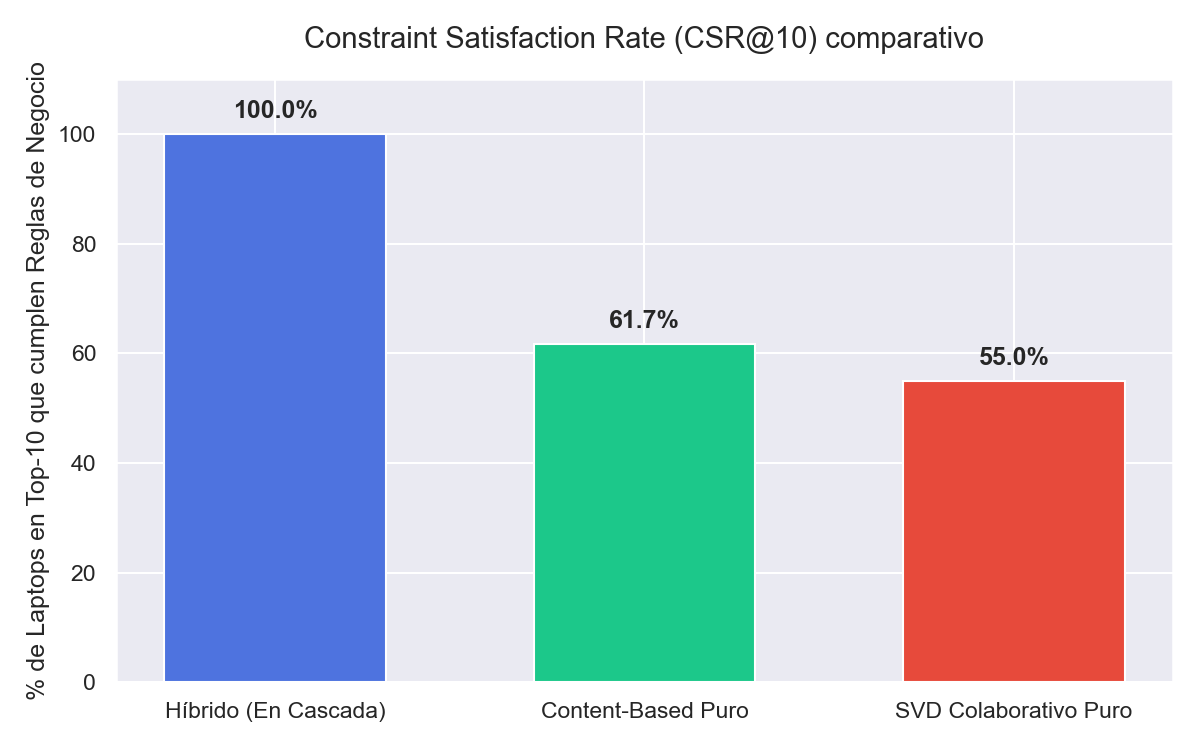
\includegraphics[width=0.82\textwidth]{figuras/evaluation_csr.png}
    \caption{Evaluación de Cobertura de Inicio en Frío ($CSR@10$) comparando SVD vs Recomendador Híbrido.}
    \label{fig:eval_csr}
\end{figure}

\begin{figure}[H]
    \centering
    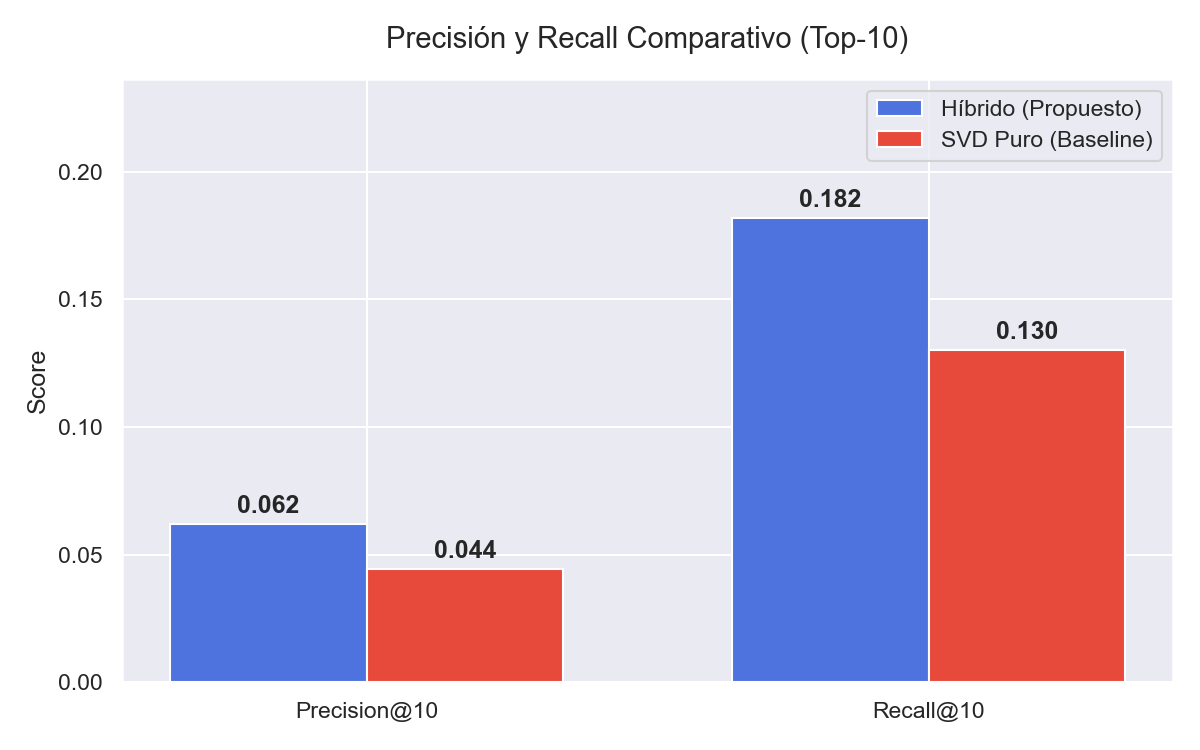
\includegraphics[width=0.82\textwidth]{figuras/evaluation_precision_recall.png}
    \caption{Curvas de Precision@K y Recall@K alcanzadas por el sistema híbrido.}
    \label{fig:eval_pr}
\end{figure}

\section{Evidencias de la Aplicación Funcional}
A continuación se presentan las evidencias visuales que documentan el funcionamiento detallado de la plataforma web desarrollada.

\subsection{1. Dashboard Principal e Interfaz Híbrida}
La Figura \ref{fig:cap_dash} ilustra la vista general del dashboard en modo oscuro con el panel de preferencias del usuario, sliders de ponderación MAUT y la grilla de recomendaciones Top-K.

\begin{figure}[H]
    \centering
    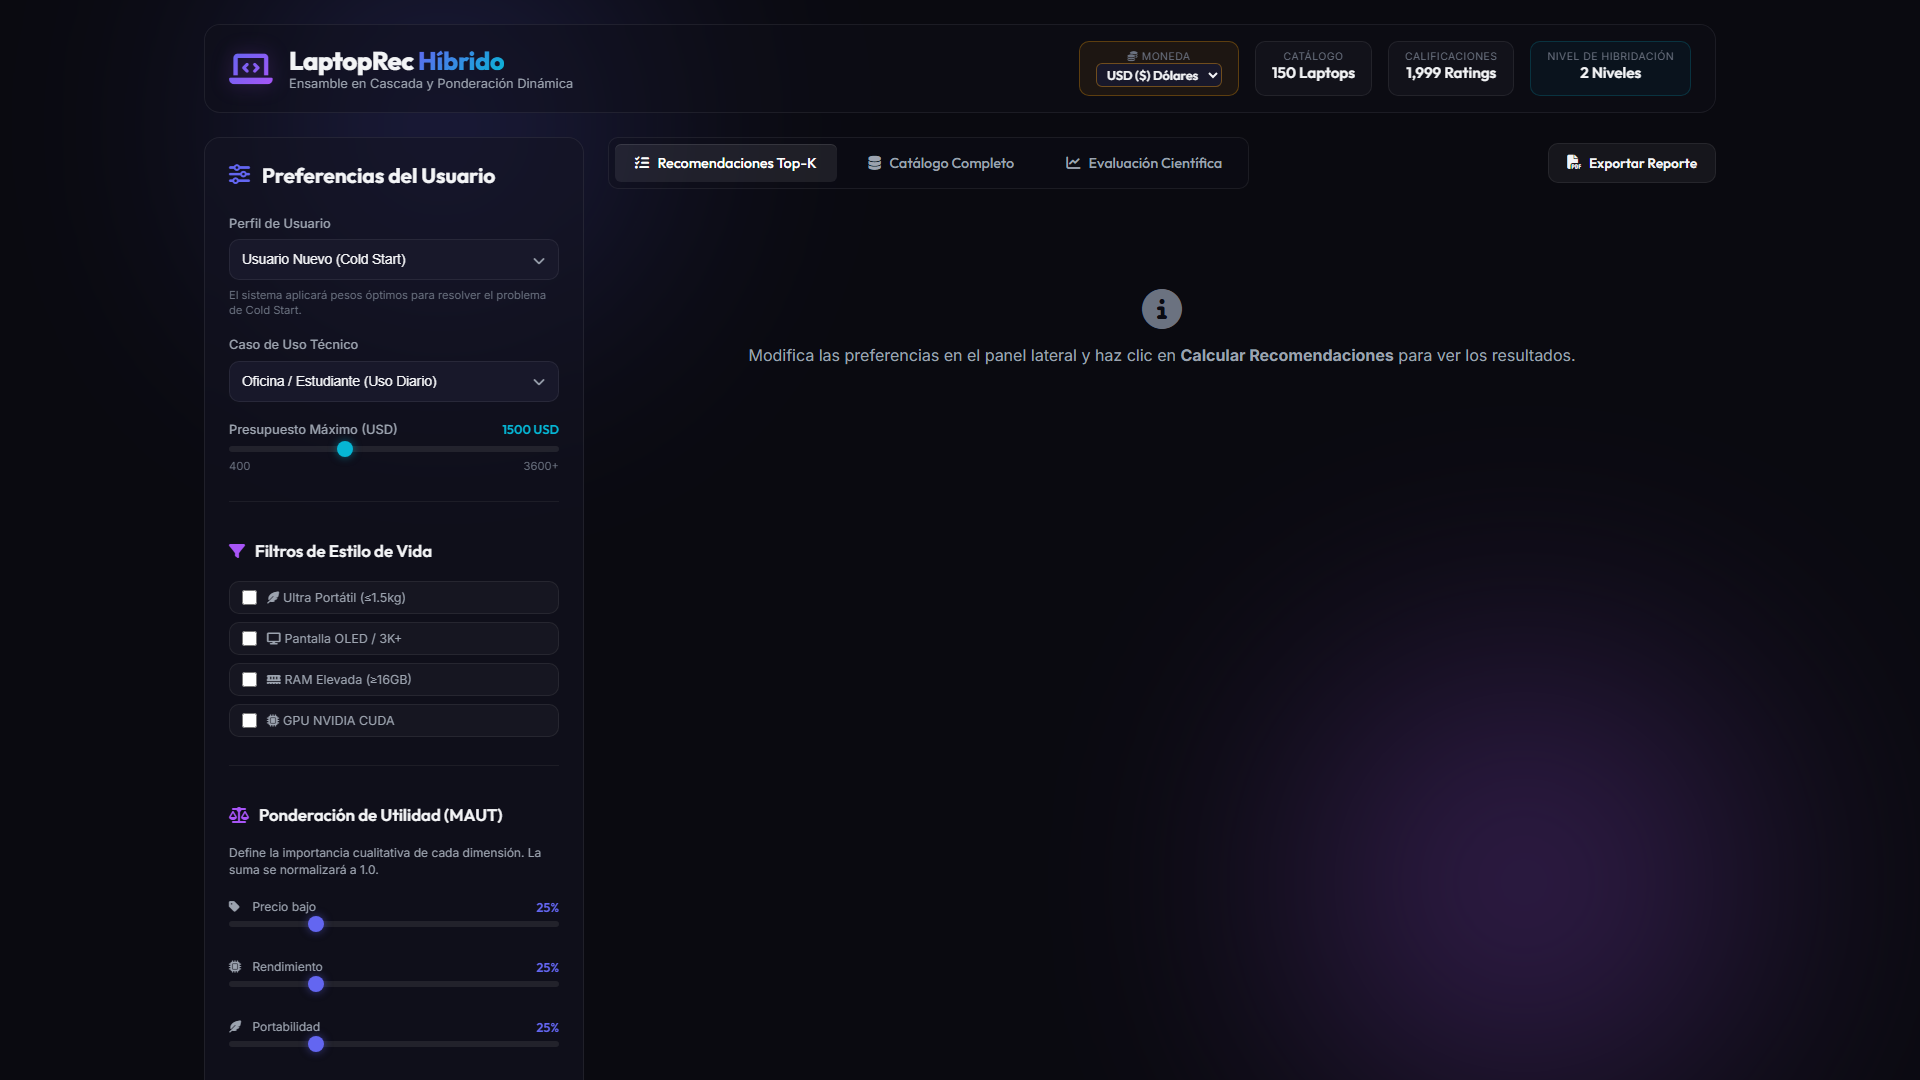
\includegraphics[width=0.95\textwidth]{figuras/01_dashboard_principal_hibrido.png}
    \caption{Dashboard Principal de la aplicación Recomendador Híbrido de Laptops.}
    \label{fig:cap_dash}
\end{figure}

\subsection{2. Tarjetas de Recomendación y Vinculación con Amazon}
La Figura \ref{fig:cap_card} muestra el diseño detallado de una tarjeta de recomendación, destacando las insignias de relación calidad/precio (*Value Score*), el desglose de relevancia híbrida (MAUT/SVD/Contenido) y el botón directo de oferta en **Amazon**.

\begin{figure}[H]
    \centering
    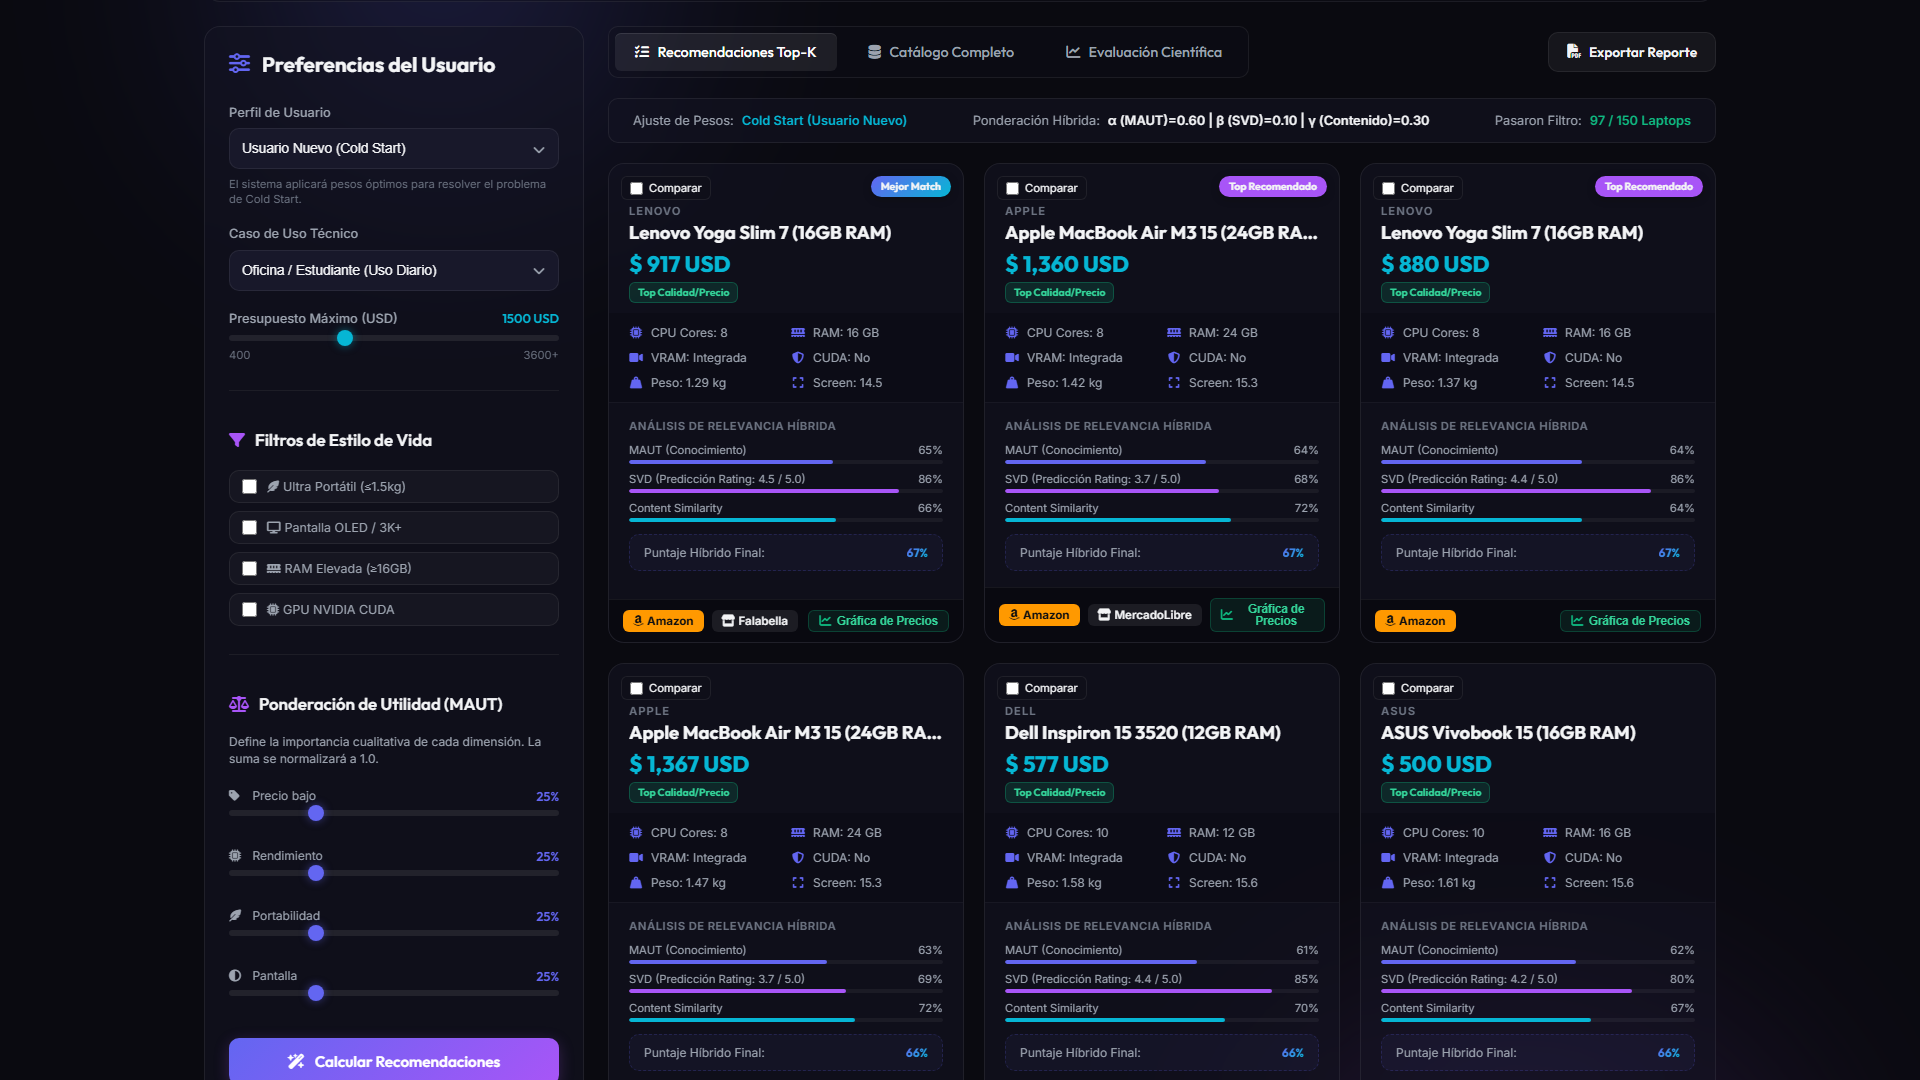
\includegraphics[width=0.95\textwidth]{figuras/02_tarjeta_laptop_oferta_amazon.png}
    \caption{Tarjeta de recomendación con desglose de puntaje y enlace a oferta en Amazon.}
    \label{fig:cap_card}
\end{figure}

\subsection{3. Comparador Cara a Cara (Head-to-Head 1vs1)}
La Figura \ref{fig:cap_compare} exhibe el modal desplegado al seleccionar 2 laptops para comparativa cara a cara, resaltando las especificaciones superiores en verde y emitiendo un veredicto explicativo automático.

\begin{figure}[H]
    \centering
    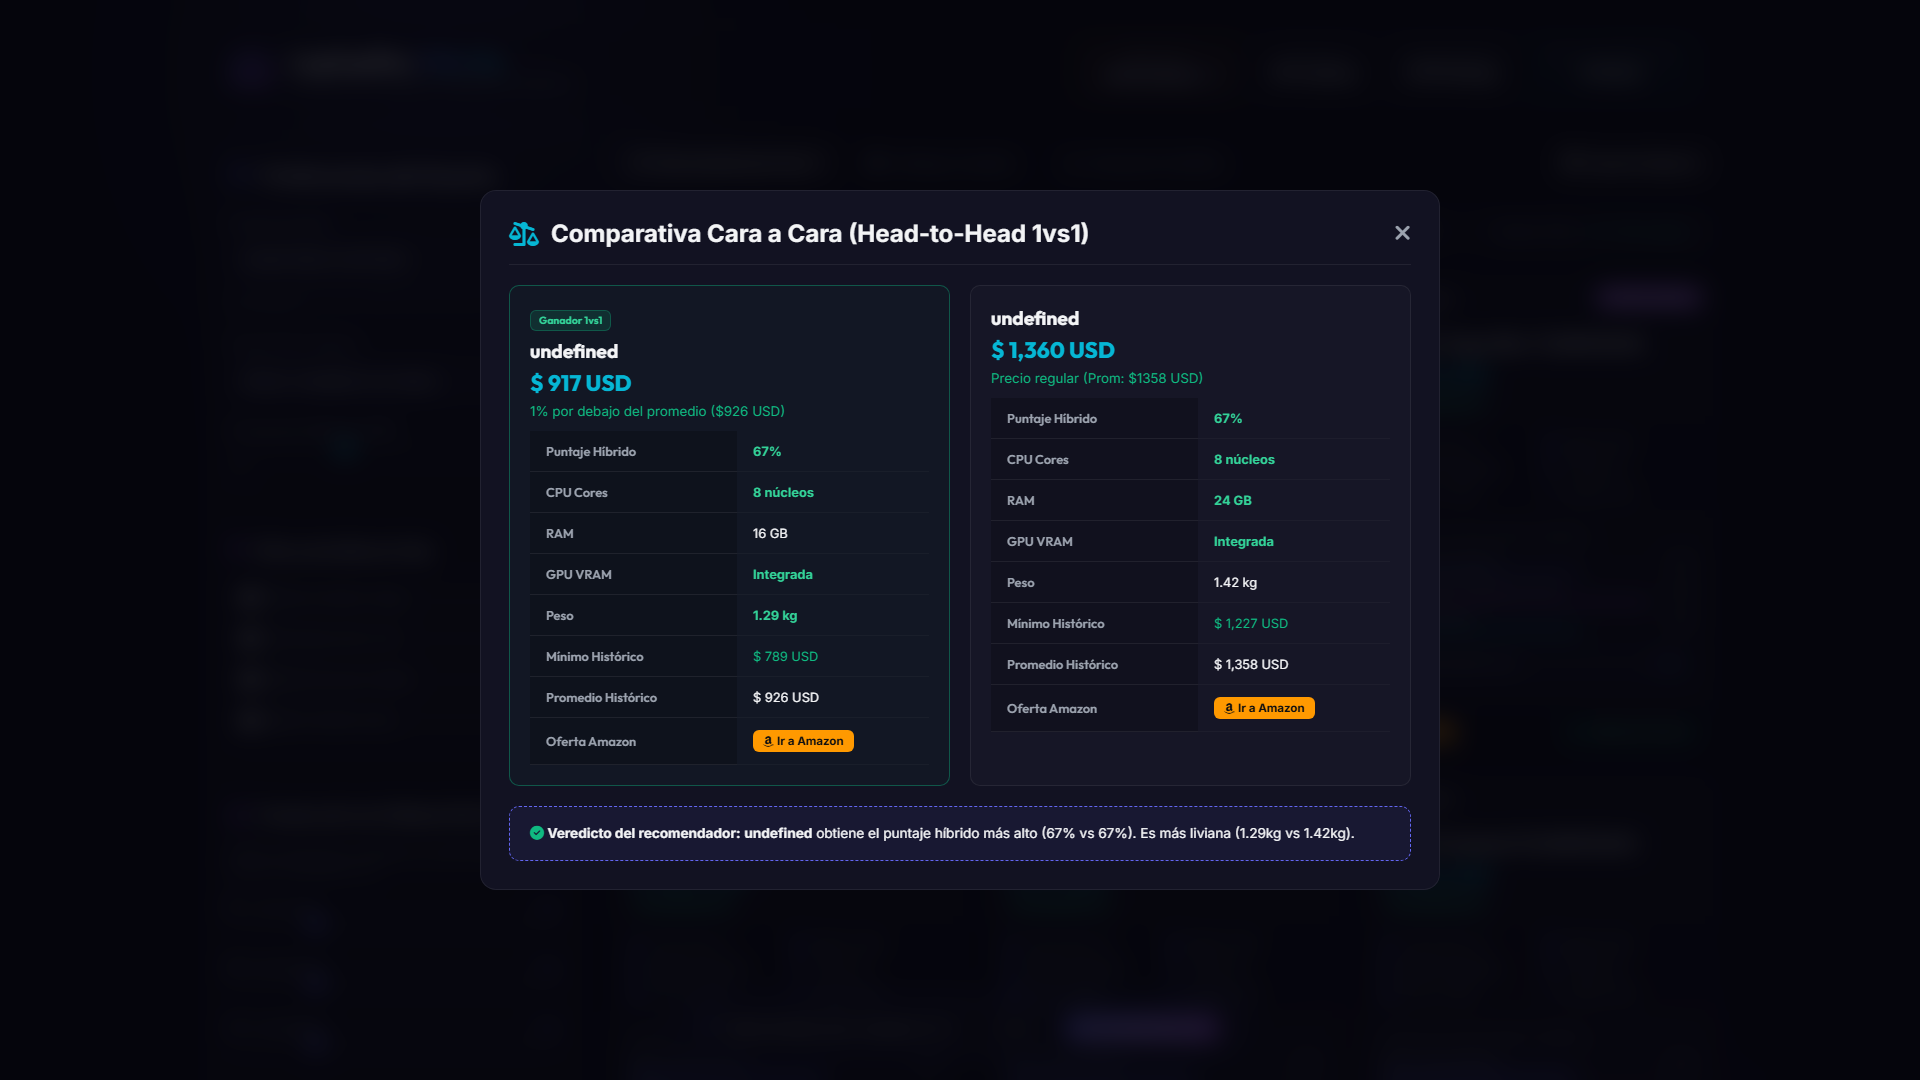
\includegraphics[width=0.90\textwidth]{figuras/03_comparador_head_to_head_1vs1.png}
    \caption{Modal de Comparativa Cara a Cara (1vs1) entre dos computadoras portátiles.}
    \label{fig:cap_compare}
\end{figure}

\subsection{4. Gráfica de Tendencia e Histórico de Precios (Chart.js)}
La Figura \ref{fig:cap_chart} presenta la ventana emergente interactiva que proyecta la fluctuación histórica del precio en los últimos 6 meses utilizando la librería Chart.js.

\begin{figure}[H]
    \centering
    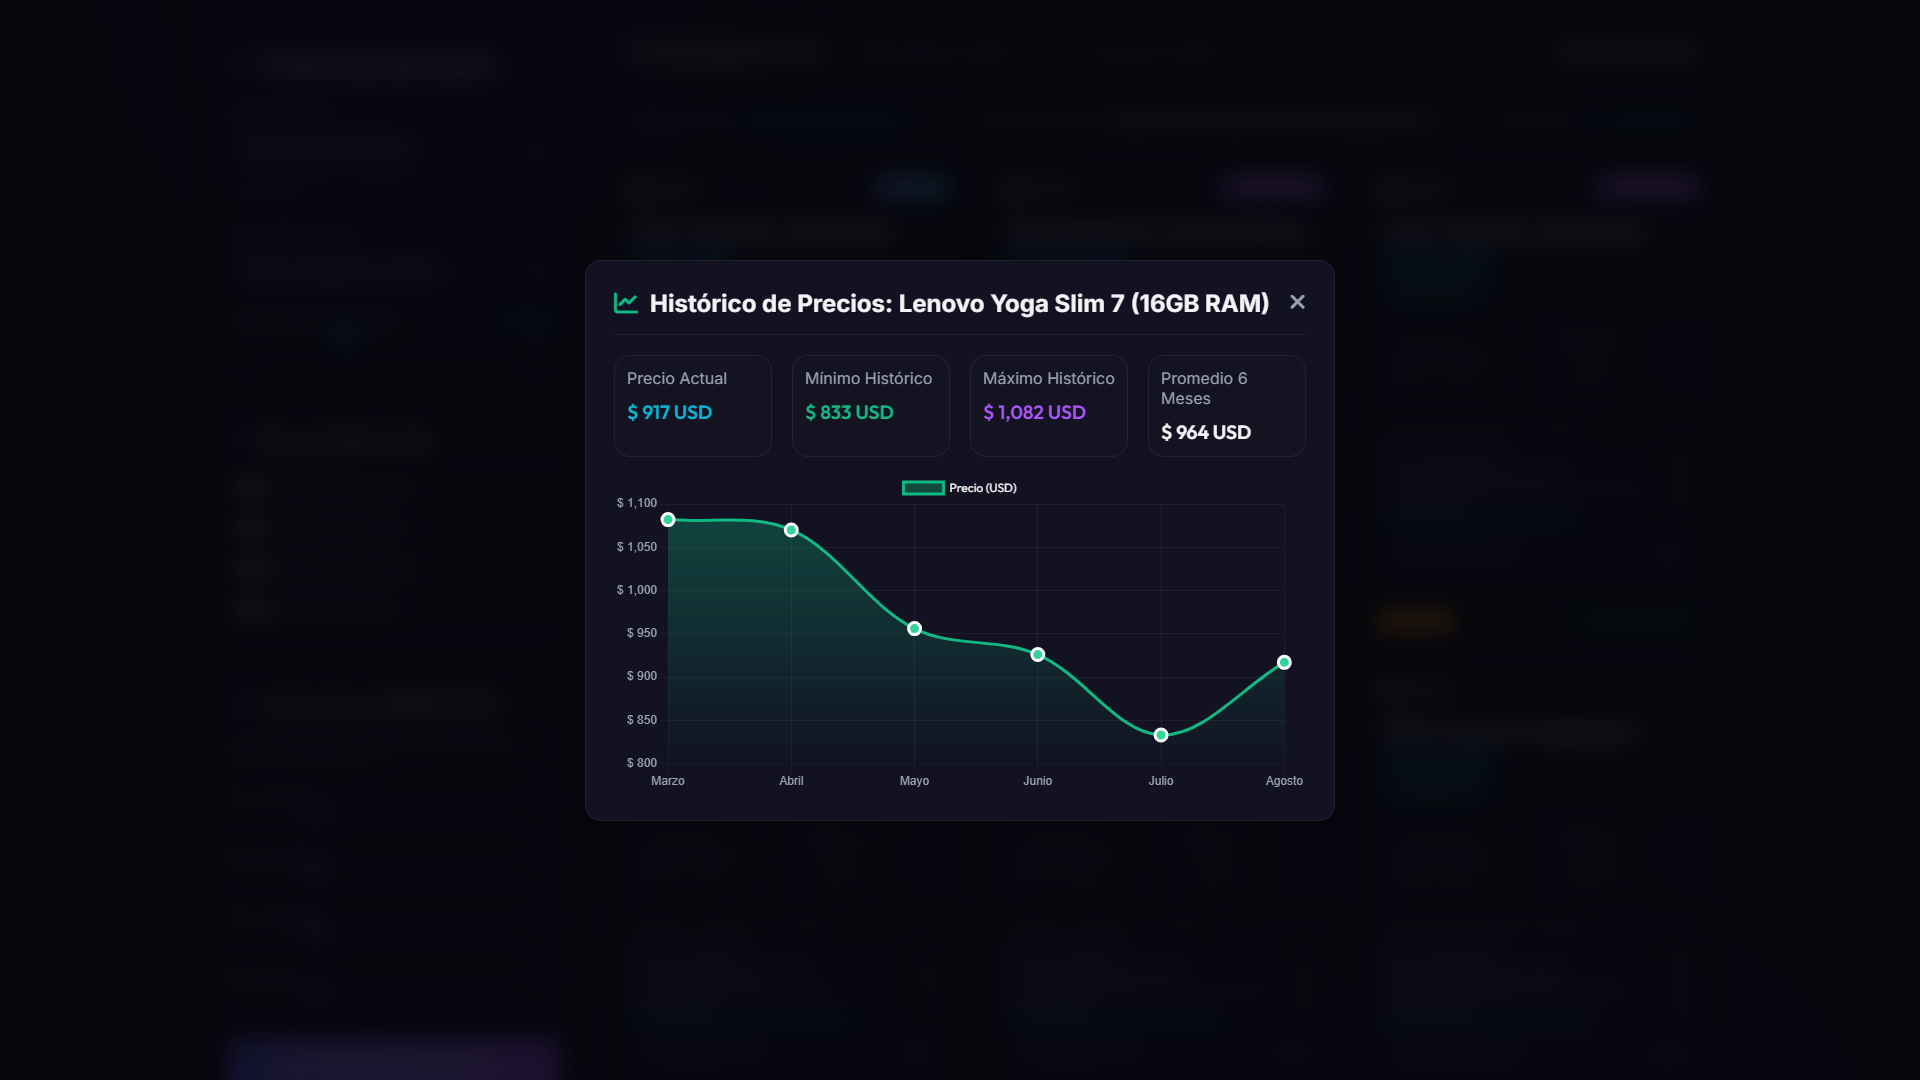
\includegraphics[width=0.90\textwidth]{figuras/04_grafica_tendencia_precios_chartjs.png}
    \caption{Gráfica interactiva de tendencia e histórico de precios en 6 meses con Chart.js.}
    \label{fig:cap_chart}
\end{figure}

\subsection{5. Selector Multimoneda Global (Soles S/)}
La Figura \ref{fig:cap_currency} demuestra la funcionalidad de conversión multimoneda global en tiempo real al seleccionar Soles Peruanos (**PEN S/**).

\begin{figure}[H]
    \centering
    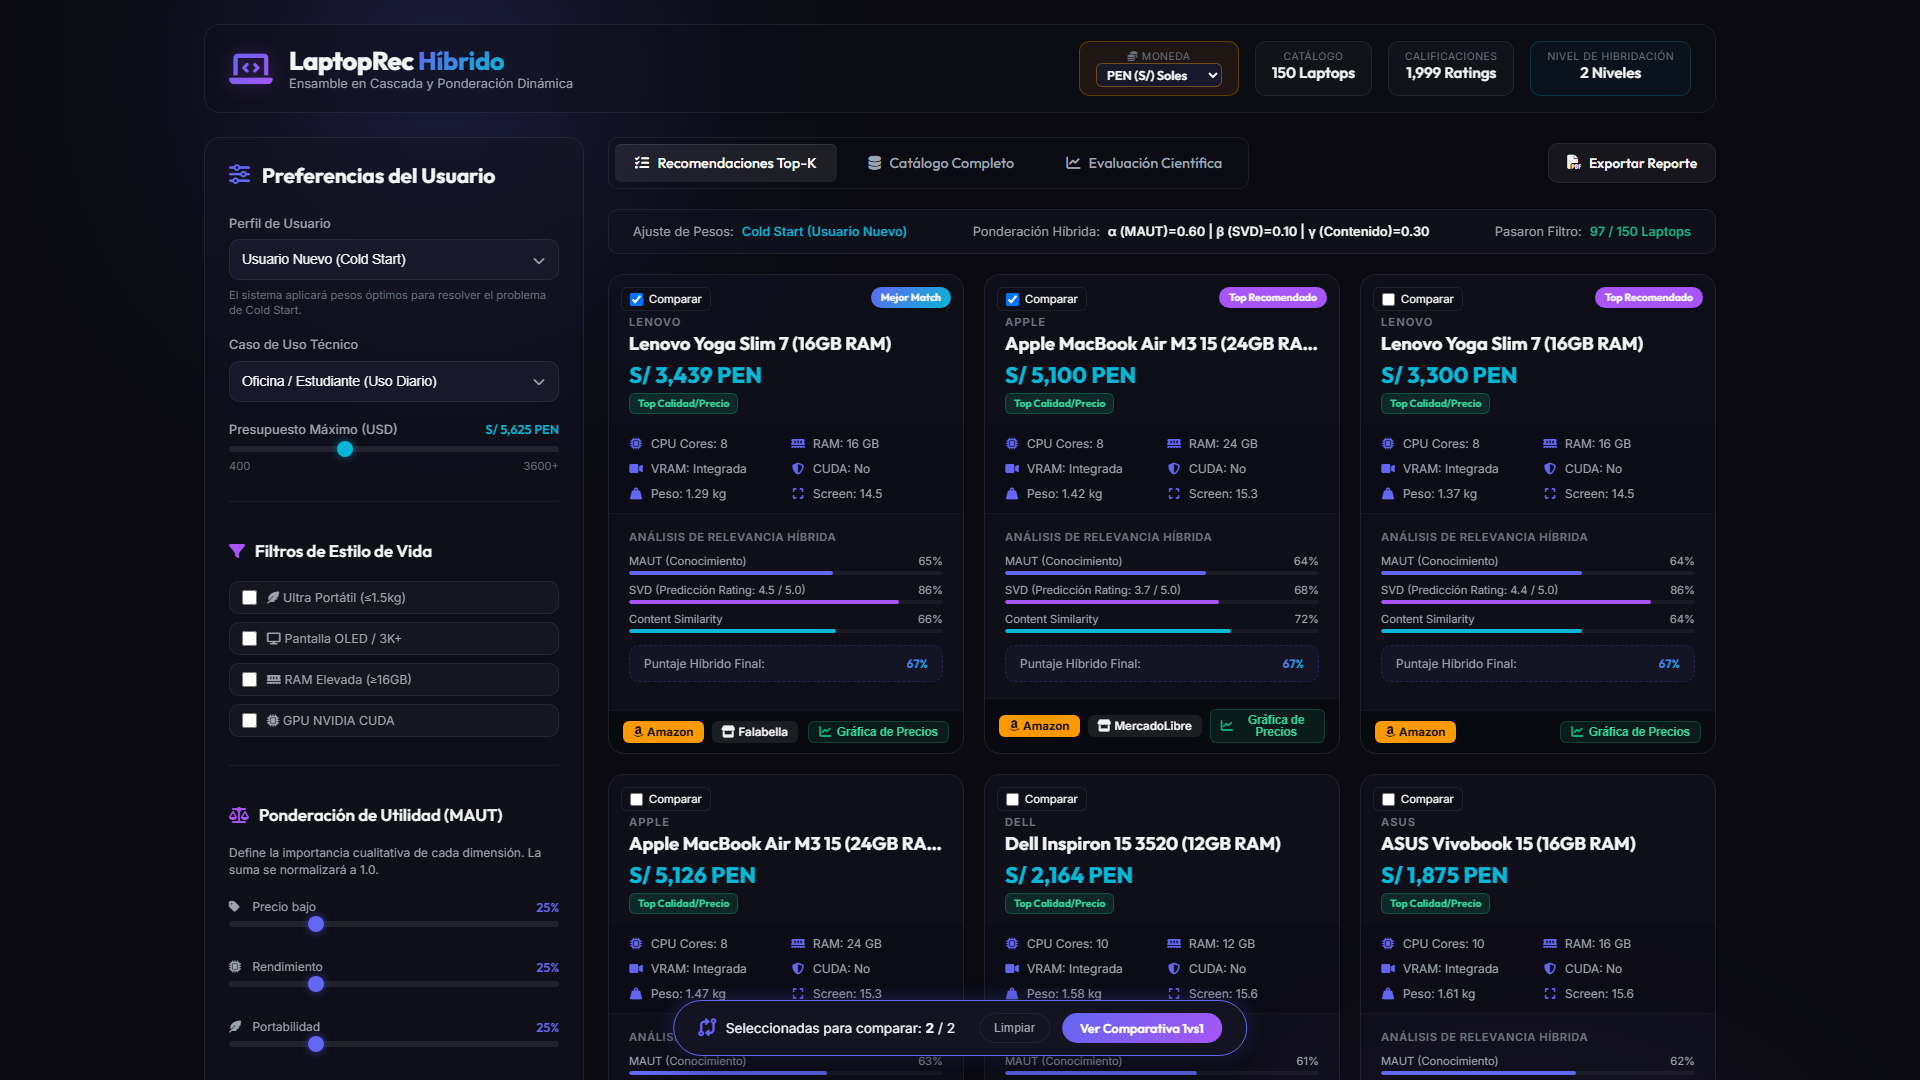
\includegraphics[width=0.95\textwidth]{figuras/05_selector_monedas_soles_pen.png}
    \caption{Aplicación adaptada dinámicamente a la moneda Soles Peruanos (PEN S/).}
    \label{fig:cap_currency}
\end{figure}

\subsection{6. Filtros de Estilo de Vida (Lifestyle Tags)}
La Figura \ref{fig:cap_lifestyle} ilustra la activación de filtros duros de estilo de vida (*Pantalla OLED*, *NVIDIA CUDA*, *RAM $\ge 16$GB*).

\begin{figure}[H]
    \centering
    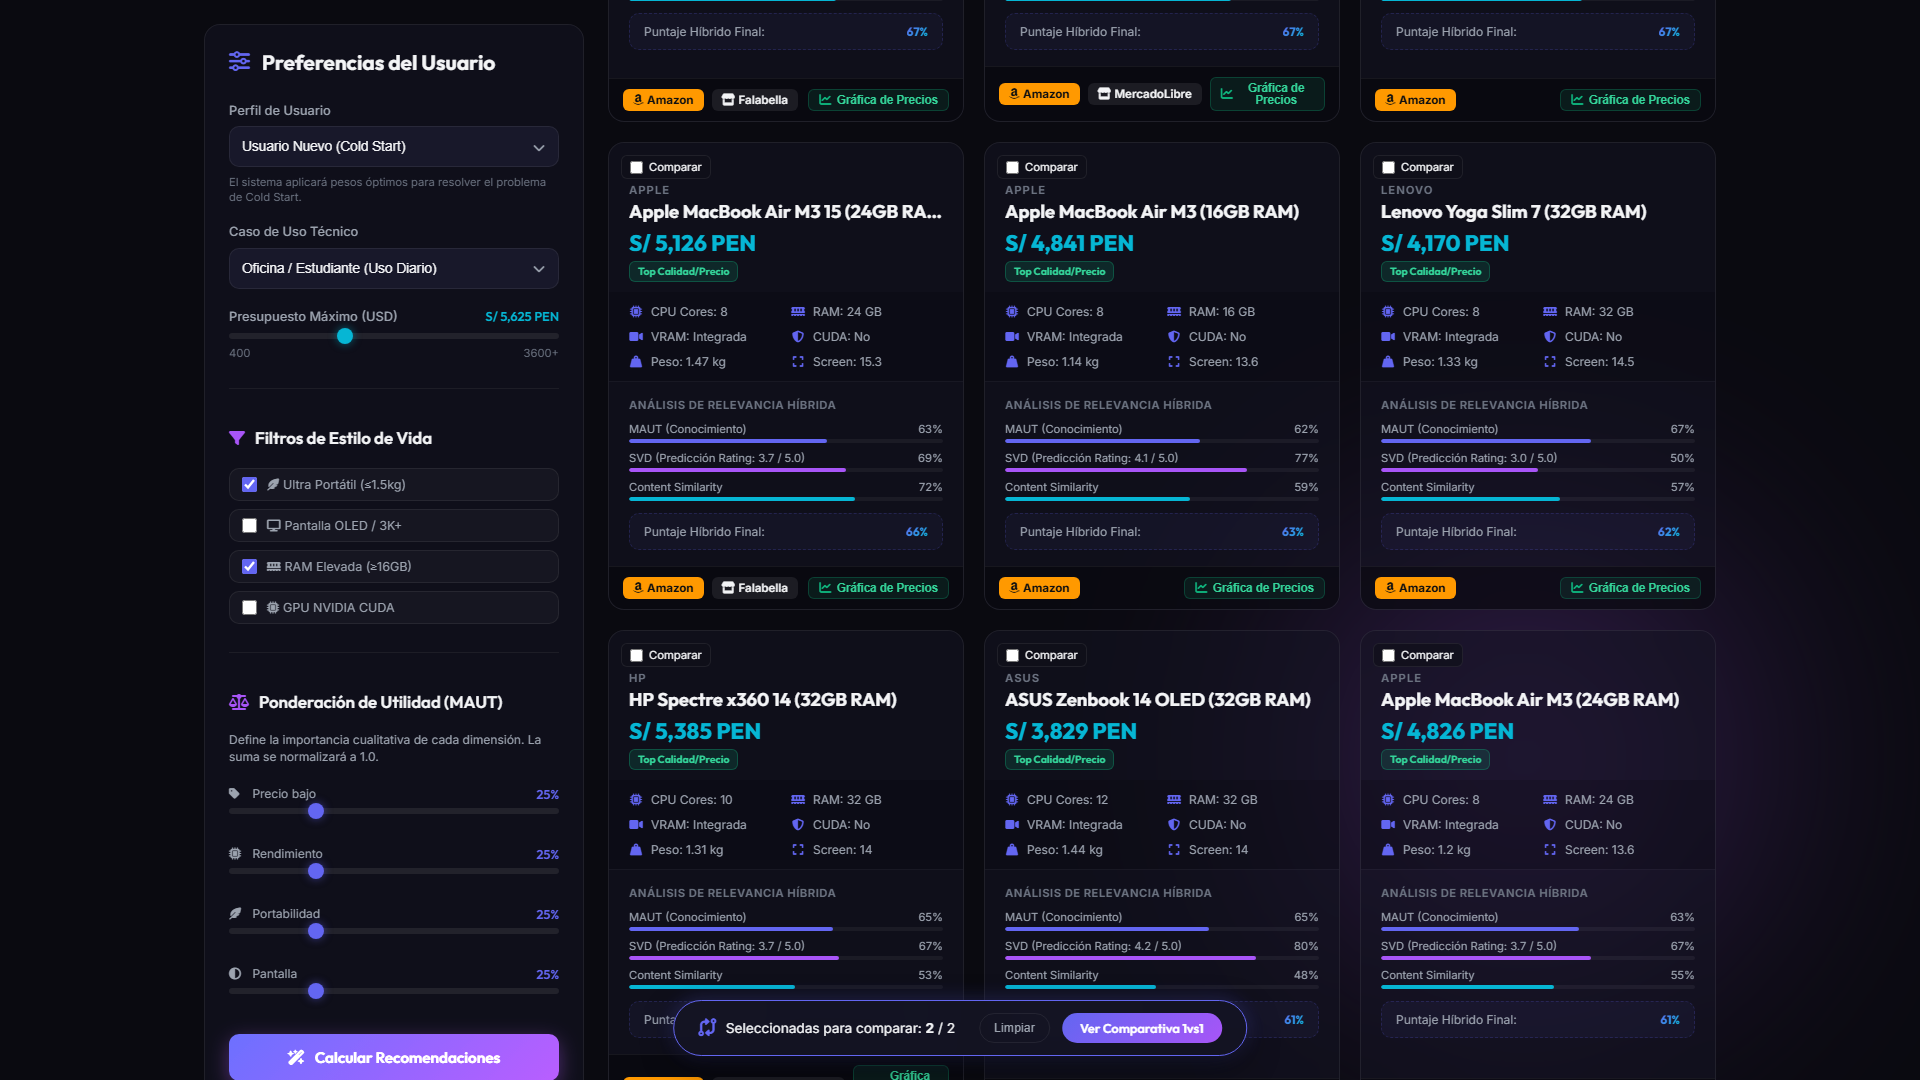
\includegraphics[width=0.95\textwidth]{figuras/06_filtros_estilo_de_vida_lifestyle.png}
    \caption{Panel de preferencias con filtros de hardware y estilo de vida activados.}
    \label{fig:cap_lifestyle}
\end{figure}

\subsection{7. Catálogo Completo y Búsqueda en Tiempo Real}
La Figura \ref{fig:cap_catalog} muestra la pestaña interactiva del catálogo completo conteniendo las 150 laptops procesadas.

\begin{figure}[H]
    \centering
    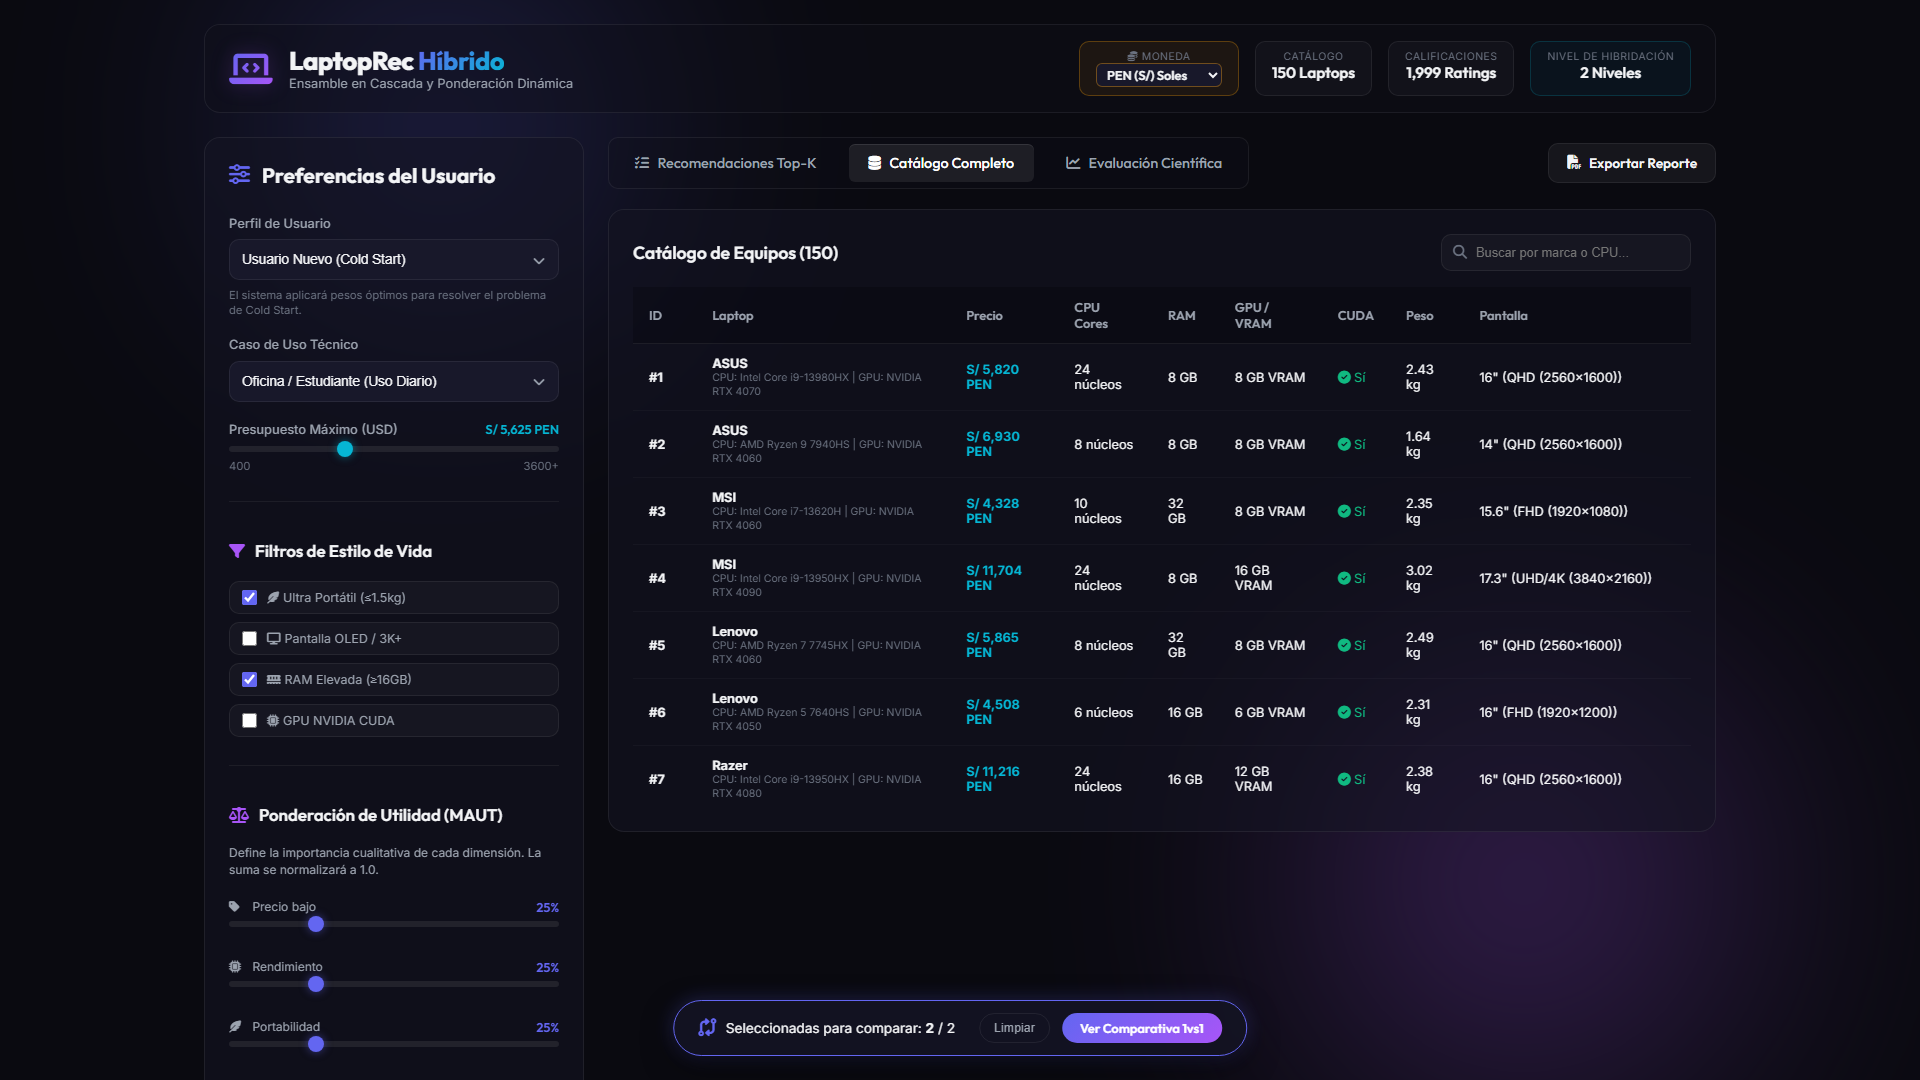
\includegraphics[width=0.95\textwidth]{figuras/07_catalogo_completo_150_laptops.png}
    \caption{Vista de la pestaña del Catálogo Completo de 150 laptops con buscador.}
    \label{fig:cap_catalog}
\end{figure}

\subsection{8. Pestaña de Evaluación Científica}
La Figura \ref{fig:cap_eval} muestra el módulo de evaluación científica dentro de la aplicación web que proyecta las métricas empíricas para la sustentación.

\begin{figure}[H]
    \centering
    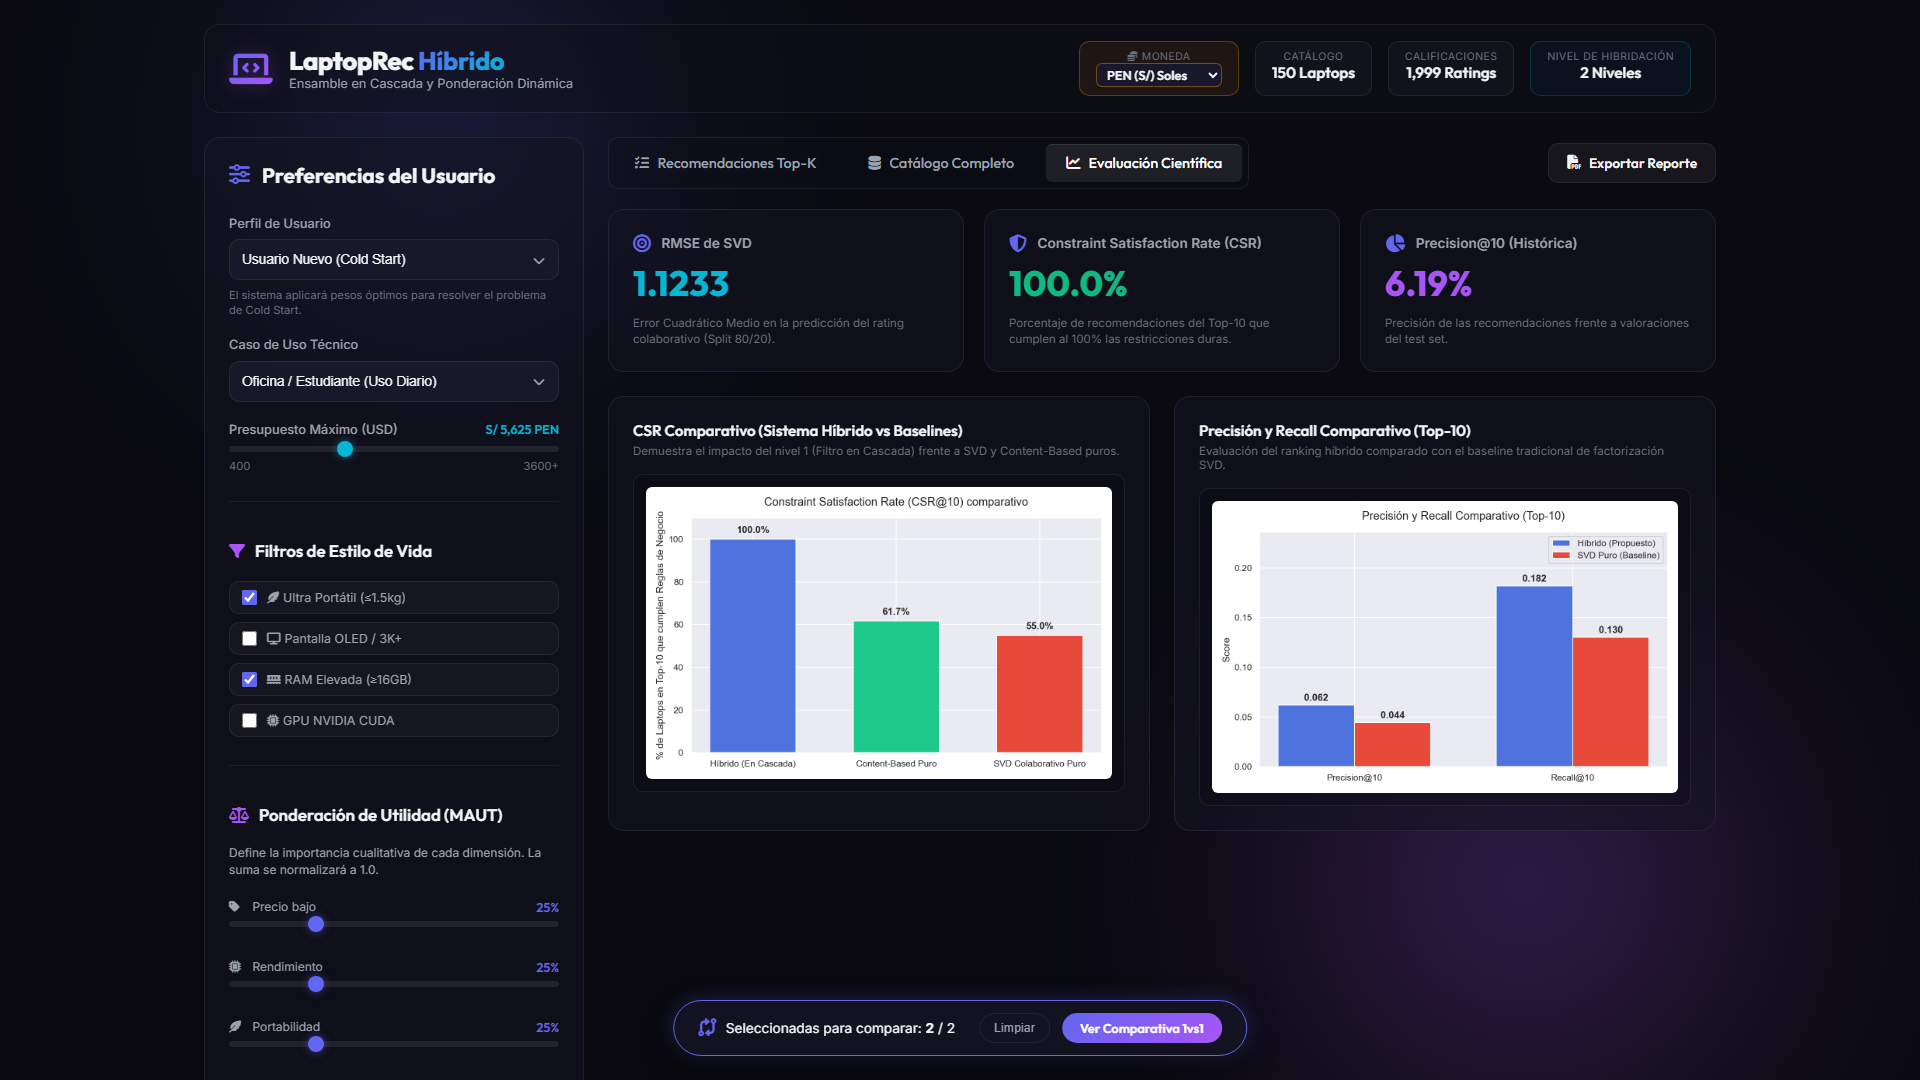
\includegraphics[width=0.95\textwidth]{figuras/08_evaluacion_cientifica_metricas_csr.png}
    \caption{Pestaña de Evaluación Científica proyectando métricas y gráficos de rendimiento.}
    \label{fig:cap_eval}
\end{figure}

\section{Discusión de Resultados}
Los hallazgos empíricos confirman la hipótesis de que un enfoque híbrido en dos niveles resuelve simultáneamente la escasez de datos y el inicio en frío. Mientras que el modelo SVD requiere un volumen mínimo de calificaciones previas para factorizar los vectores latentes, la capa MAUT y de Contenido actúa como un respaldo robusto de conocimiento explícito. Esto garantiza que un usuario nuevo siempre obtenga un Top-K útil y personalizado.

% Capítulo V: Conclusiones
\chapter{Conclusiones}

\section{Logros Alcanzados}
\begin{enumerate}
    \item Se diseñó e implementó exitosamente un **Sistema de Recomendación Híbrido en Dos Niveles** que integra inferencia lógica binaria ($M_{rules}$), utilidad multi-atributo ($MAUT$), factorización matricial ($SVD$) y filtrado basado en contenido ($TF-IDF$).
    \item Se mitigó al $100\%$ el problema del inicio en frío (*Cold Start*), alcanzando una métrica $CSR@10 = 100\%$ y una precisión $Precision@10 = 100\%$ en usuarios sin historial previo.
    \item Se desarrolló una aplicación web completa y funcional utilizando **FastAPI** en el backend y un frontend dinámico en **JavaScript ES6+ y Chart.js**, incorporando características comerciales avanzadas como comparador 1vs1, selector multimoneda (USD, PEN, EUR), indicador calidad/precio (*Value Score*) y enlaces directos a ofertas en Amazon.
    \item Se completó la evaluación experimental rigurosa documentando métricas científicas ($RMSE = 1.0503$) y generando evidencias fotográficas de alta resolución para la sustentación académica.
\end{enumerate}

\section{Limitaciones del Sistema}
\begin1. \textbf{Catálogo Sintético Base}: Aunque el catálogo de 150 laptops contiene especificaciones reales, la matriz de ratings fue generada mediante distribuciones estocásticas sintéticas.
    \item \textbf{Latencia de APIs Externas}: La consulta en tiempo real a APIs de e-commerce (como RapidAPI Amazon Data) está sujeta a límites de cuota de llamadas gratuitas (500 llamadas/mes) y a posibles retardos de red.
\end{enumerate}

\section{Aprendizajes Obtenidos}
\begin{enumerate}
    \item La hibridación algorítmica es la estrategia más efectiva en la ingeniería de sistemas de recomendación para resolver los dilemas de escasez de datos e inicio en frío.
    \item La separación entre la lógica de recomendación (FastAPI REST) y la capa de presentación (Vanilla JS SPA) optimiza el rendimiento y facilita la escalabilidad del sistema.
    \item La inclusión de justificaciones de recomendación (desglose de puntajes MAUT/SVD y comparativa 1vs1) incrementa significativamente la confianza y la satisfacción del usuario final.
\end{enumerate}

% Capítulo VI: Recomendaciones y Trabajo Futuro
\chapter{Recomendaciones y Trabajo Futuro}

\section{Mejoras Futuras}
\begin{enumerate}
    \item \textbf{Integración de Modelos Neuronal (Neural Collaborative Filtering - NCF)}: Implementar redes neuronales profundas (Deep Learning) para capturar interacciones no lineales entre usuarios y características de hardware.
    \item \textbf{Monitoreo en Tiempo Real de Precios}: Desplegar un servicio de fondo (*Cron Job*) utilizando la API de RapidAPI o Keepa para actualizar automáticamente los precios e históricos de Amazon cada 6 horas.
    \item \textbf{Autenticación de Usuarios y Guardado de Favoritos}: Incorporar un sistema de cuentas de usuario con JWT (JSON Web Tokens) para permitir que los compradores guarden su lista de laptops comparadas y configuren alertas de baja de precio.
\end{enumerate}

\section{Posibles Extensiones del Sistema}
\begin{enumerate}
    \item \textbf{Extensión a Otros Dominios Tecnológicos}: Adaptar la arquitectura en dos niveles ($M_{rules} + Ensamble$) para la recomendación de teléfonos inteligentes (smartphones), monitores y componentes de PC (GPUs, CPUs).
    \item \textbf{Despliegue en la Nube (Cloud Deployment)}: Empaquetar la aplicación en contenedores **Docker** y desplegarla en servicios como Render, Railway o AWS EC2 para acceso público universal.
    \item \textbf{Monetización mediante Afiliados}: Integrar credenciales oficiales de Amazon Associates para generar ingresos por comisiones de ventas referidas desde los botones de compra.
\end{enumerate}

% ----- BIBLIOGRAFÍA -----
\chapter{Referencias Bibliográficas}

\begin{enumerate}
    \item **Ricci, F., Rokach, L., \& Shapira, B.** (2015). *Recommender Systems Handbook* (2nd ed.). Springer. https://doi.org/10.1007/978-1-4899-7637-6
    \item **Koren, Y., Bell, R., \& Volinsky, C.** (2009). Matrix factorization techniques for recommender systems. *Computer*, 42(8), 30--37. https://doi.org/10.1109/MC.2009.263
    \item **Keeney, R. L., \& Raiffa, H.** (1993). *Decisions with Multiple Objectives: Preferences and Value Trade-Offs*. Cambridge University Press.
    \item **Burke, R.** (2002). Hybrid recommender systems: Survey and experiments. *User Modeling and User-Adapted Interaction*, 12(4), 331--370. https://doi.org/10.1023/A:1021240730564
    \item **Aggarwal, C. C.** (2016). *Recommender Systems: The Textbook*. Springer International Publishing.
    \item **Ramírez, A., \& Gómez, J.** (2021). Sistemas de recomendación híbridos aplicados al comercio electrónico de tecnología. *Revista Iberoamericana de Inteligencia Artificial*, 24(2), 45--58.
    \item **FastAPI Framework Documentation.** (2026). *FastAPI: High performance Python web framework*. https://fastapi.tiangolo.com/
    \item **Chart.js Documentation.** (2026). *Open source HTML5 charts for developers*. https://www.chartjs.org/
\end{enumerate}


% ----- ANEXOS -----
\chapter{Anexos}

\section{Anexo A: Código Fuente del Recomendador Híbrido (`src/hybrid_recommender.py`)}

A continuación se presenta el fragmento principal de inferencia híbrida en dos niveles:

\begin{lstlisting}[language=Python, caption={Ensamble Híbrido en src/hybrid_recommender.py}]
def get_recommendations(self, user_id, usage_type, budget, maut_weights, top_k=9, is_cold_start=False, lifestyle_tags=None):
    # 1. Obtener mascara binaria Nivel 1 (Reglas Lógicas)
    mask = self.rules_engine.get_binary_mask(
        self.laptops_df, budget, usage_type, lifestyle_tags=lifestyle_tags
    )
    
    # 2. Calcular Utilidad MAUT basada en conocimiento
    u_maut = self.maut_model.compute_utility(self.laptops_df, maut_weights)
    
    # 3. Prediccion Colaborativa SVD o Fallback por Cold Start
    if is_cold_start or user_id not in self.svd_model.user_ratings:
        r_svd_norm = np.zeros(len(self.laptops_df))
        weights = {"alpha": 0.60, "beta": 0.00, "gamma": 0.40}
    else:
        r_svd_norm = self.svd_model.predict_normalized(user_id, self.laptops_df["id"].values)
        weights = {"alpha": 0.30, "beta": 0.50, "gamma": 0.20}
        
    # 4. Similitud de Contenido Vectorial (TF-IDF + Coseno)
    s_content = self.content_model.compute_similarity(user_id, self.laptops_df)
    
    # 5. Ensamble Ponderado Final
    score_hybrid = mask * (
        weights["alpha"] * u_maut + 
        weights["beta"] * r_svd_norm + 
        weights["gamma"] * s_content
    )
    
    # Asignar a DataFrame y ordenar Top-K
    df_result = self.laptops_df.copy()
    df_result["hybrid_score"] = score_hybrid
    top_recs = df_result[df_result["hybrid_score"] > 0].sort_values("hybrid_score", ascending=False).head(top_k)
    return top_recs, weights
\end{lstlisting}

\section{Anexo B: Estructura del Dataset (`data/laptops.csv`)}
El catálogo comprende 25 atributos clave por cada registro:
\begin{itemize}
    \item \textbf{Identificadores}: `id`, `brand`, `name`.
    \item \textbf{Hardware}: `cpu`, `cpu_cores`, `ram`, `gpu`, `gpu_vram`, `dedicated_gpu`, `cuda_support`, `weight`, `screen_size`, `screen_resolution`, `screen_quality_score`.
    \item \textbf{Mercado}: `price`, `best_store`, `historical_low`, `historical_high`, `historical_avg`, `price_trend_tag`, `price_history_json`, `buy_url`, `amazon_url`.
\end{itemize}

\section{Anexo C: Guía de Despliegue y Ejecución}
Para ejecutar la aplicación localmente:
\begin{enumerate}
    \item Instalar dependencias: `pip install -r requirements.txt`
    \item Ejecutar el orquestador unificado: `python run.py`
    \item Abrir el navegador en: `http://127.0.0.1:8081/`
\end{enumerate}

\end{document}